\chapter{Introduction}
\label{cha:introduction}

% Most enterprise tools nowadays support multiple companies as users. And of course for organization each company needs to have their own sepparate space to work in

% The focus of this thesis, is to propose and implement a multi-tenant feature for Management System of PROCEED.
% PROCEED(PROCess EnginE in a Distributed environment) is a BPMN process engine.
% BPMN is an abstraction used to model business logic. 
% PROCEED has a Management System, where users can manage their BPMN models.
% Environments allow users to manage everything that PROCEED offers with a layer of separation, meaning that, the contents of each environments, are separate to all other environments.

% Nowadays cloud applications have become very popular in professional settings.
% Cloud applications are those, which are served and accessed over the internet, they offer many benefits:

In today's digital age, businesses heavily rely on cloud applications
to work on their assets, e.g. documents, spreadsheets, and presentations.
Cloud applications are software tools that are accessed and run entirely over the internet.
Typically, an instance of the application runs on a computer in a data center,
and users access it through a web browser or a dedicated application.
These tools represent a paradigm shift from traditional software applications,
where the majority of the work was done on the user's device.
Shifting a part, or even all the workload to a cloud application offers many advantages:

\begin{itemize}
	\item Accessibility: They can be accessed anywhere from anywhere with an internet connection.
	\item Cost-Efficient: Most cloud applications implement a payment structure, where
	      users pay based on how much they use.
	\item Data safety: All files are stored by the application in the cloud, and they don't
	      have to be stored in the user's device, which could be lost, stolen or damaged.
	      % users don't have to implement their own data storage solutions,
	      % which may be insecure.
	\item Collaboration: Typically, collaboration is easier since everything can be found
	      in one place, instead of having to send files back and forth.
	\item Device-agnostic: Many cloud applications can be accessed through different device types.
	\item No IT overhead: Users don't have to set up the application on their own, which would require technical knowledge.
\end{itemize}

\begin{figure}[H]
	\centering
	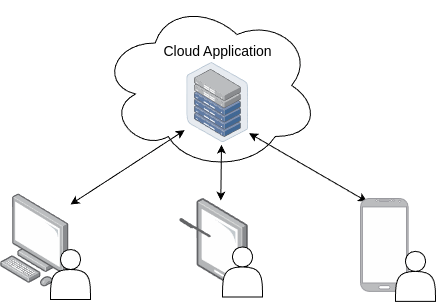
\includegraphics[scale=0.35]{images/basic-cloud-services.drawio.png}
	\caption{Users can access cloud applications from any device with an internet connection.}
	\label{fig:cloud-applications}
\end{figure}

% A key selling point of these, is that companies don't have to do any technical work setting the software up, they can pay for a subscription and start using the tool right away, either through a browser or by installing an executable on their computer.
% A very important technical aspect for such tools, that enables the ease of use, is the ability to support multiple companies using them at once.

% Most of these benefits only apply if all users interact with the same cloud application.
% This means that the users interact with what appears to them to be a single application
% This is called multi-tenancy, and it is implemented by most popular cloud applications, e.g. by Teams, Slack, Asana, and many more.
% A tenant can be seen as an entity that uses the application, which can be either a single user or an organization made up of many users.

One very common feature that makes these benefits possible is called \textit{multi tenancy}.
\textit{multi tenancy} is a software architecture in which one single instance of an application
can be used by multiple users or organizations at the same time.
Without \textit{multi tenancy}, each user or organization would need to run the application on
their own computers,
negating most of the benefits listed earlier.

% means that many different users or organizations can use the same cloud application at the same
% time, even though it looks like they each have their own private version.

% NOTE: maybe take this out
Think of an application that supports \textit{multi tenancy} like a big apartment building.
Each tenant (user or organization) has their
own private apartment (their space), where they store their belongings (their assets).
Every tenant is living in the same building (cloud application), but each tenant has their
own private space.

Many popular cloud applications use this approach. For example, when you use Microsoft Teams,
Slack, or Asana, you're sharing the application with many other companies, but you only
see and interact with your own team.

% \begin{figure}[H]
% 	\centering
% 	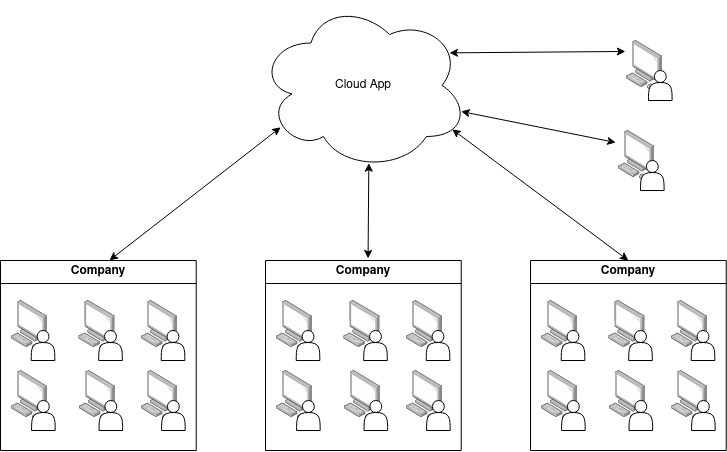
\includegraphics[scale=0.45]{images/mt-cloud-services.png}
% 	\caption{Multi tenancy in cloud applications: the same instance of the cloud
% 		application, can be used by different tenants, with different structures, without them knowing about each other.}
% 	\vspace{-1em} % Negative value to remove space
% 	\label{fig:multi-tenant=cloud-applications}
% \end{figure}

PROCEED %(short for PROCess EnginE in a Distributed environment)% is a cloud application,
is a Business Process Management System,
it uses BPMN at its core to model and execute business processes.
%For readers unfamiliar with BPMN, 
%it can be thought of as a powerful flowchart that can be used to describe any conceivable process.
BPMN (Business Process Model and Notation) is a standardized graphical notation used for documenting business processes.
BPMN is typically used inside of organizations to illustrate sequences of tasks,
decision points, and interactions within various business processes, providing a standardized visual representation.

PROCEED offers two products:
\begin{itemize}
	\item Distributed Process Engine (DPE for short): the DPEs execute BPMN processes.
	\item Management System (MS for short): the MS is a cloud application that gives users
	      a graphical interface to work on their BPMN processes and deploy these to the DPEs.
\end{itemize}

\begin{figure}[H]
	\centering
	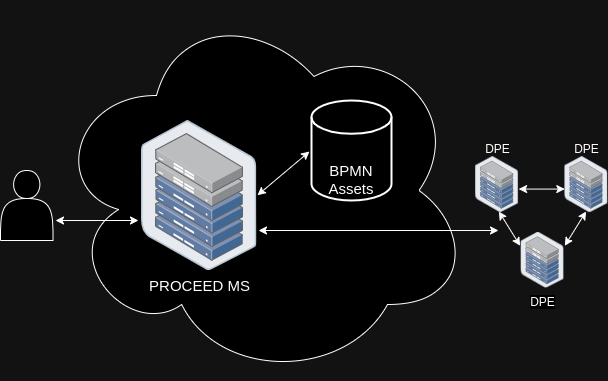
\includegraphics[scale=0.45]{images/quick-ms-overview.drawio.png}
	\caption{Overview of PROCEED: users interact with the Management System, to create and
		manage BPMN models. The Management System has the ability to deploy these models to the Distributed Process Engines.}
	\label{fig:proceed-overview}
	\vspace{-1em} % Negative value to remove space
\end{figure}

%Throughout this thesis we'll refer to any information that a user can access as an asset.
%Also all actions that a user can perform in the PROCEED Management System, are viewed as an action performed on an asset.

%The PROCEED Management system encompasses various asset types, which can be categorized as follows:
%\begin{enumerate}
%    \item BPMN models: Processes, Projects, and Templates are assets that can be created in PROCEED, that fall into the category of BPMN models.
%    Although each one of them stores slightly different information and carries a distinct semantic meanings, they all have BPMN at their core.
%    \item Execution related assets: Tasklist, Executions and Machines are all assets related to the execution of a BPMN model.
%end{enumerate}

% TODO !!

Currently the MS lacks full multi-tenancy support, it only supports individual users and
doesn't fully support organizations.
For organizations to be supported, members of the organization need to be able to have a
shared workspace, where they can work on the same assets.
% This could technically achieved if members of the organization shared all assets with
% each other.
However, PROCEED only supports universal sharing, meaning that all users would be able to
see the shared assets.
Furthermore, even if it was possible to share assets only to a group of users, it would be
very cumbersome and error-prone.
% This means that organizations, where multiple people work together are not supported by the
% MS.
% For this reason, it presents many difficulties for organizations, as there is no convenient way for multiple members of the organization to work together on assets in the MS.
% For this reason, the MS is not suitable for organizations, as there is no convenient way
% for multiple members of an organization to work together.
% Furthermore, any admin user in the MS has the right to view and modify every asset, which presents privacy risks for organizations.
% The only somewhat viable option for organizations to use PROCEED, is to run the server
% code of the MS on their own computers, which renders most benefits of cloud applications void.
%This is because all assets are stored in a central database without a good way to isolate them from other tenants.
%The only information that BPMN related assets are stored with, that helps towards isolating them from other tenants is the owner and a set of labels.

For this reason, this thesis implements multi-tenant functionality into the PROCEED MS by introducing the concept of Environments.
The MS should be able to hold multiple isolated environments, where tenants can work on their assets.
% Each tenant should be able to work in their own isolated environment, which lives in a central instance of the Management System. 
Each user, who signs in, should automatically have their own Environment, this allows users to work on
personal projects.
Organizations should be able to create environments where multiple members can work together.
Additionally, environments should include a folder structure to improve the organization of
assets.
% Currently the MS only provides labels for organizing assets.
% Assets can be labeled with one or more labels, which can be used to filter assets. 
% Users cannot add, delete nor modify these labels.
% Folders will provide more flexibility than labels.

\begin{figure}[H]
	\centering
	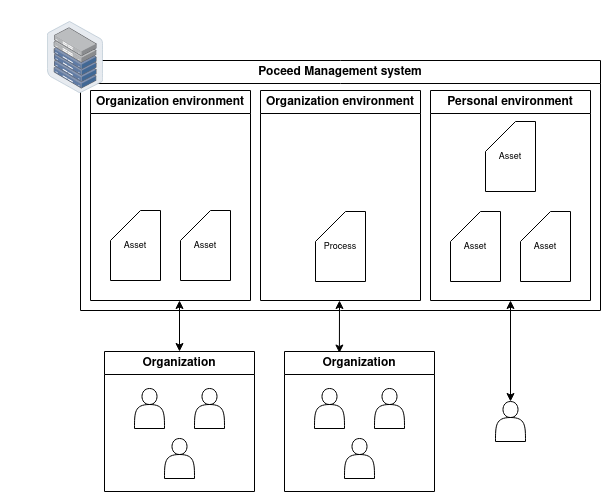
\includegraphics[scale=0.45]{images/proceed-workspaces-v2.drawio.png}
	\caption{Goal of this thesis: tenants can work in their own isolated environments in
		the PROCEED Management System.}
	\label{fig:proceed-envitonments-overview}
\end{figure}

% These labels symbolize, what department the process belongs to. 

%Access to assets in the MS is restricted through roles,
%so that one of three scenarios can happen to a user:
%
%\begin{itemize}
%    \item The user doesn't permissions to see assets.
%    \item The user has permission to view assets, but isn't an admin. In case, the user would only be able to see his own assets.
%    \item The user is an admin and can see all assets.
%\end{itemize}
%
%This low level of granularity makes the PROCEED Management System unsuitable hosting multiple tenants, since all their assets would be stored in the same fashion, and the only way for users to see assets that weren't created by them, would be to grant them the admin role.
%Granting users the admin role, would in turn mean that they would be able to see all BPMN Assets, which poses privacy concerns for tenants, since other tenants could potentially access their assets.

%When it comes to Execution related assets, Machines and Executions also have similar problems to BPMN assets, since these need to be private for each company.

%This makes it so, that if more than one tenant wants to use PROCEED they're left with few options:
%
%\begin{itemize}
%\end{itemize}
%Each company would have to spin up their own self hosted version of PROCEED.
%
%Both of these options have considerable downsides. 
%No separation between companies is a hindrance to privacy and each company having to spin up an instance of PROCEED is a big barrier to entry.
%This makes it very hard to scale PROCEED to be able to be comfortably used by multiple companies.
%
% \begin{figure}[H]
%    \centering
%    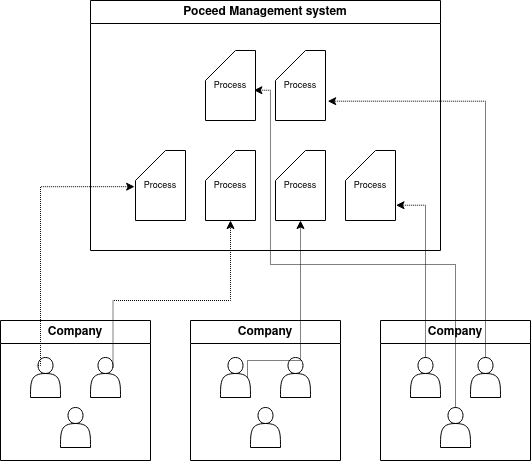
\includegraphics[scale=0.5]{./images/proceed-no-workspaces.drawio.png}
%    \caption{PROCEED Management System with no multi-tenant support.}
%    \label{fig:PROCEED-no-Environments}
% \end{figure}


% Research questions
\section{Research Questions}
\label{cha:researchquestions}

For environments to be successfully integrated into the PROCEED Management System,
a few important questions need to be addressed.
These questions will help ensure that environments work smoothly with the existing database structure,
role system, and user management. By answering them, we can ensure the implementation is effective and doesn’t
disrupt the current system.


\begin{enumerate}
	% Data Modeling and Architecture

	\item Environment representation: How can we model environments and their hierarchical
	      folder structure within the MS's storage solution to ensure the following:
	      \begin{itemize}
		      \item Data integrity: find a schema that facilitates data consistency after updates.
		      \item Asset-Environment association: find a schema that associates assets with their
		            respective environments while maintaining a clear and consistent data model.
		      \item Efficiency: find a schema that allows to efficiently query the database.
	      \end{itemize}

	\item How do users have to be managed to best allow them to be members of multiple environments?

	\item How can organizations model their hierarchical structures within environments
	      to allow members of the organization to have different levels of access to assets?
	      % \item How can we extend the existing PROCEED role system to incorporate
	      %   environment-specific permissions?

	      % Roles and Permissions
	\item How can users work on personal Projects outside an organization.


	      % \item What mechanisms are needed to ensure that role-based access control is consistently enforced?

	\item How can the Management System allow users to manage assets on different
	      environments?

	      % Usability and Developer Experience

	      % \item What user interface elements and interaction patterns are most effective for navigating and managing folders and environments?

	      % \item How can we minimize the impact on existing code while ensuring seamless integration?

	      % Additional Considerations

	      % Performance and Scalability: How will the addition of environments impact the performance and scalability of the PROCEED Management System? What optimizations can be made to ensure that the system remains responsive and efficient even with a large number of users and environments?
	      % Migration Strategies: How can we seamlessly migrate existing PROCEED data and users into the new environment-based structure? What strategies can we employ to minimize disruption during the transition?
	      % Security: What additional security measures are needed to protect data within environments? How can we prevent unauthorized access to environments and their assets?
\end{enumerate}

% Task List

\section{Task List}
\label{cha:tasklist}

The following task list outlines the concrete steps necessary to address the research
questions and ensure a successful implementation of environments.
Each task is designed to tackle specific aspects of the MS's
architecture, user management, and role assignments.

% private environment
% Functional / non functional
% can / must / should 
% TODO: 
% \item What software abstractions (e.g., classes, interfaces, functions) can we create to simplify the process of identifying and managing a user's environment in the backend code? 

\begin{enumerate}
	\item The MS has to support environments, isolated spaces where users can work on their
	      assets. \label{cha:tasklist:item-environments}
	      \begin{enumerate}
		      \item Every asset in the MS \ref{cha:relatedwork:proceed-assets} must be stored in only one environment.

		      \item Assets stored in one environment can only be accessed by members of that
		            environment.

		      \item Environments must have a hierarchical folder system to store assets.
		            \begin{enumerate}
			            \item Find a suitable abstraction to represent folders in a database
			                  that facilitates consistency after updates and is fast to query.

			            \item Ensure privacy between environments.

			                  % escribir aca ya que tiene que haber herencia
			                  % reescribir should be modified no es tan fuerte/
			                  % likely redundant

			                  % depending on the folder the asset is in.
		            \end{enumerate}

		            % NOTE: replace concurrently with eaesier word
		      \item The MS must be able to hold multiple environments and let users access them concurrently.

	      \end{enumerate}
	      % ---------------------------------------------------------------------------------------
	      % ---------------------------------------------------------------------------------------

	      %write about how there are personal and organization environments
	\item Implement personal and organization environments. While both are environments
	      and share common functionality as described in
	      \ref{cha:tasklist:item-environments}, they must behave differently in some
	      situations.
	      \begin{enumerate}
		      \item Personal environments can only have one member.

		      \item Personal environments can only store Processes and Folders.

		      \item Organization environments support all assets described in \ref{cha:relatedwork:proceed-assets}.

		      \item Organization environments can have a name and description.

		      \item Organization environments must support multiple members, i.e. multiple users can
		            work on the assets stored inside of it.

		      \item Organization environments must have a role system, where roles can be assigned to
		            users, to manage their access to assets.

		      \item Users of organization environments that have right permissions must be able to invite users
		            to the organization environment.
	      \end{enumerate}


	\item The MS's user management has to be adapted to fit environments: before the
	      implementation of this thesis, users where strictly tied to one instance of the MS,
	      meaning each time a new instance of the MS was created, a new user storage had to be
	      configured.
	      \begin{enumerate}
		      \item Users have to be global, meaning that they don't belong to any environment.

		      \item Implement Guest users.
		            \begin{enumerate}
			            \item Allow users to try the MS without signing in with their personal
			                  information.
			            \item Guest users can sign in with their personal information and become a normal
			                  user.
			            \item Guest users can transfer their assets to a normal user.

			            \item Guest users can not create or be part of organization environments.
		            \end{enumerate}

		            % TODO: does this belong here?
		      \item Every user has to have a personal environment.

		            % TODO: does this belong here?
		      \item Personal environments must be tightly coupled with users, i.e. when a user is
		            deleted so is his personal environment.
	      \end{enumerate}


	\item The MS's preexisting role system must be adapted to fit organization environments
	      and their folder structure:
	      The MS already has a role system in place to manage users' access to resources,
	      this has to be adapted to work with organization environments.
	      \begin{enumerate}
		      \item Roles must belong to only one organization environment.
		      \item The role system must be replicated for each environment, i.e. it works the
		            same as before, with the difference that it is now specific to an environment.
		            E.g. if a role allowed a user to manage all processes before the implementation of
		            environments, now, with the same role, he will be able to modify all processes
		            inside the organization environment the role belongs to.
		      \item Find a suitable permission inheritance model for roles based on the folder
		            structure of an environment (e.g. a user with a role in a parent
		            folder, has the same permissions in all subfolders).
		      \item Ensure roles are always enforced in the backend.
		      \item The frontend UI must adapt to a user's roles, by only showing options that the user has permission to do.
	      \end{enumerate}
\end{enumerate}

The following are non-functional requirements that have to be met for the implementation
of environments in the MS.
The goal of these is to ensure that the implementation is user-friendly and most
importantly developer-friendly, as many developers will have to work with the codebase in
the future.
This means that where possible, simple solutions should be favored over complex ones.

\begin{enumerate}
	\item Keep changes to the MS to a minimum.

	      % \item The implementation shouldn't be repetitive, the same functional components should be used for both personal and organization environments.

	\item The user interface for navigating and managing folders and environments should
	      be intuitive and easy to use.

	\item Prioritize developer experience by creating clear abstractions and APIs.
	      \begin{enumerate}
		      \item The same data structure and functions should be used for both personal and organization
		            environments where possible. E.g. the same function that creates a folder in a
		            personal environment should be used to create a folder in an organization environment.

		      \item Choose a simple data structure for the folder system, with straightforward
		            functions for modification.

		      \item Create simple abstractions for the backend code of the MS, that allow to
		            acknowledge a user's environment with minimal effort.

		      \item Create a simple abstraction for the frontend, that facilitates adapting
		            the Interface for each.
	      \end{enumerate}

	      % \item Environments should be easy to create, manage and delete.
	      %   \begin{enumerate}
	      %     \item The frontend should provide intuitive interfaces for creating and deleting organization environments.
	      %       // not functional
	      %     \item Provide well documented APIs to create, manage and delete environments both for the frontend and the backend.
	      %       needs more description. ldap
	      %     \item Environments should provide the option to import an existing user database.
	      %   \end{enumerate}
\end{enumerate}



%---------------- 
% old

% \begin{enumerate}
% \item The same data structure should be used to represent personal and organization environments.
% \begin{enumerate}
% \item Personal and organization environments should have a near identical structure.
% kann man falsch verstehen umschreiben
% \item Most of the backend and frontend code should work the same, regardless of if it is dealing with a personal or an organization environment.
% \end{enumerate}

% not functional - keine stichpunkte  - : 2 points in one paragraph

% \end{enumerate}

% The introduction of "environments" within this system is a pivotal enhancement. These environments serve as distinct, isolated spaces, ensuring that the contents and operations within each environment remain entirely separate from those in all other environments. This separation offers users the capability to manage various aspects of PROCEED's functionality while maintaining data and process integrity within their designated environment. This thesis explores the design, implementation, and implications of the multi-tenant feature within the Management System of Proceed, contributing to a more versatile and secure user experience.


% \begin{enumerate}
%     \item Interface for creatring and deleting company workspaces.
%     
%     \item Adapt roles to workspaces.
%     \begin{itemize}
%         \item Each role has to belong to one workspace
%         \item Roles have to cascade down the folder structure of workspaces
%         \item Roles have to roughly keep the same functionality as before.
%     \end{itemize}
%     
%     \item Adapt asset storage for workspaces.
%     \begin{itemize}
%         \item Find a suitable solution to store assets.
%         \item Ensure privacy between workspaces.
%     \end{itemize}
%     
%     \item Adapt the Management System's API to take into account workspaces.
%     \begin{itemize}
%         \item Make sure that a the requester specifies the workspace he is referring to.
%         \item Make sure that the requester belongs to the workspace where the asset he is trying to access is located.
%         \item Implement an endpoint for users to get the workspaces they belong to.
%         \item Implement an endpoint for users to manage the workspaces they belong to.
%     \end{itemize}
%     
%     \item The Management System frontend will only have one active workspace at a time.
%     \begin{itemize}
%         \item All actions that manipulate assets, roles or create users, will be performed on the active workspace.
%         \item Only the assets of the active workspace will be shown.
%         \item There will be a clear indication of what workspace is active
%         \item There will be an easy way to switch between workspaces.
%     \end{itemize}
%     
%     \item Interfaces for managing different aspects of company workspace's members.
%     \begin{itemize}
%         \item Option for creating and deleting users.
%         \begin{itemize}
%             \item Basic creation with manual input.
%             \item Import existing user Databases.
%         \end{itemize}
%         \item Option for inviting users to the workspace.
%         \item Option to manage users' roles.
%     \end{itemize}
%     
%     \item Users should be able to share assets.
%     \begin{itemize}
%         \item Allow users to share assets with other users.
%         \begin{itemize}
%             \item A person who shares something will be referred to as a sharer and the reciepient as a sharee
%         \end{itemize}
%         \item Users will only be able to share assets if their roles allow it.
%         \item Each shared object has associated perimissions with it, which restrict the sharee's ability to access and manipulate it.
%         \item Sharees will be able to view and select all workspaces where they have at least one shared asset.
%         \begin{itemize}
%             \item Sharees sill see the folder structure of the workspace, but they won't see any of the assets in them, besides the ones shared with him
%         \end{itemize}
%         \item The frontend will implement a Interface to share assets.
%         \item The frontend will implement a Interface to manage shares.
%         \item The frontend will indicate to the sharer, in the asset overview that an asset is shared.
%         \item Users that are allowed to view an asset will also be able to see the users that it has been shared to.
%     \end{itemize}
% \end{enumerate}
